\subsection{Solenoid and Torus Magnets}


\subsection{Geometry}
The solenoid geometry is produced with the GEMC perl api. The solenoid is a single polycone volume, shown in \F{solenoid}
in a section view with the target and an 11 GeV electron beam.

\begin{figure}
	\centering
	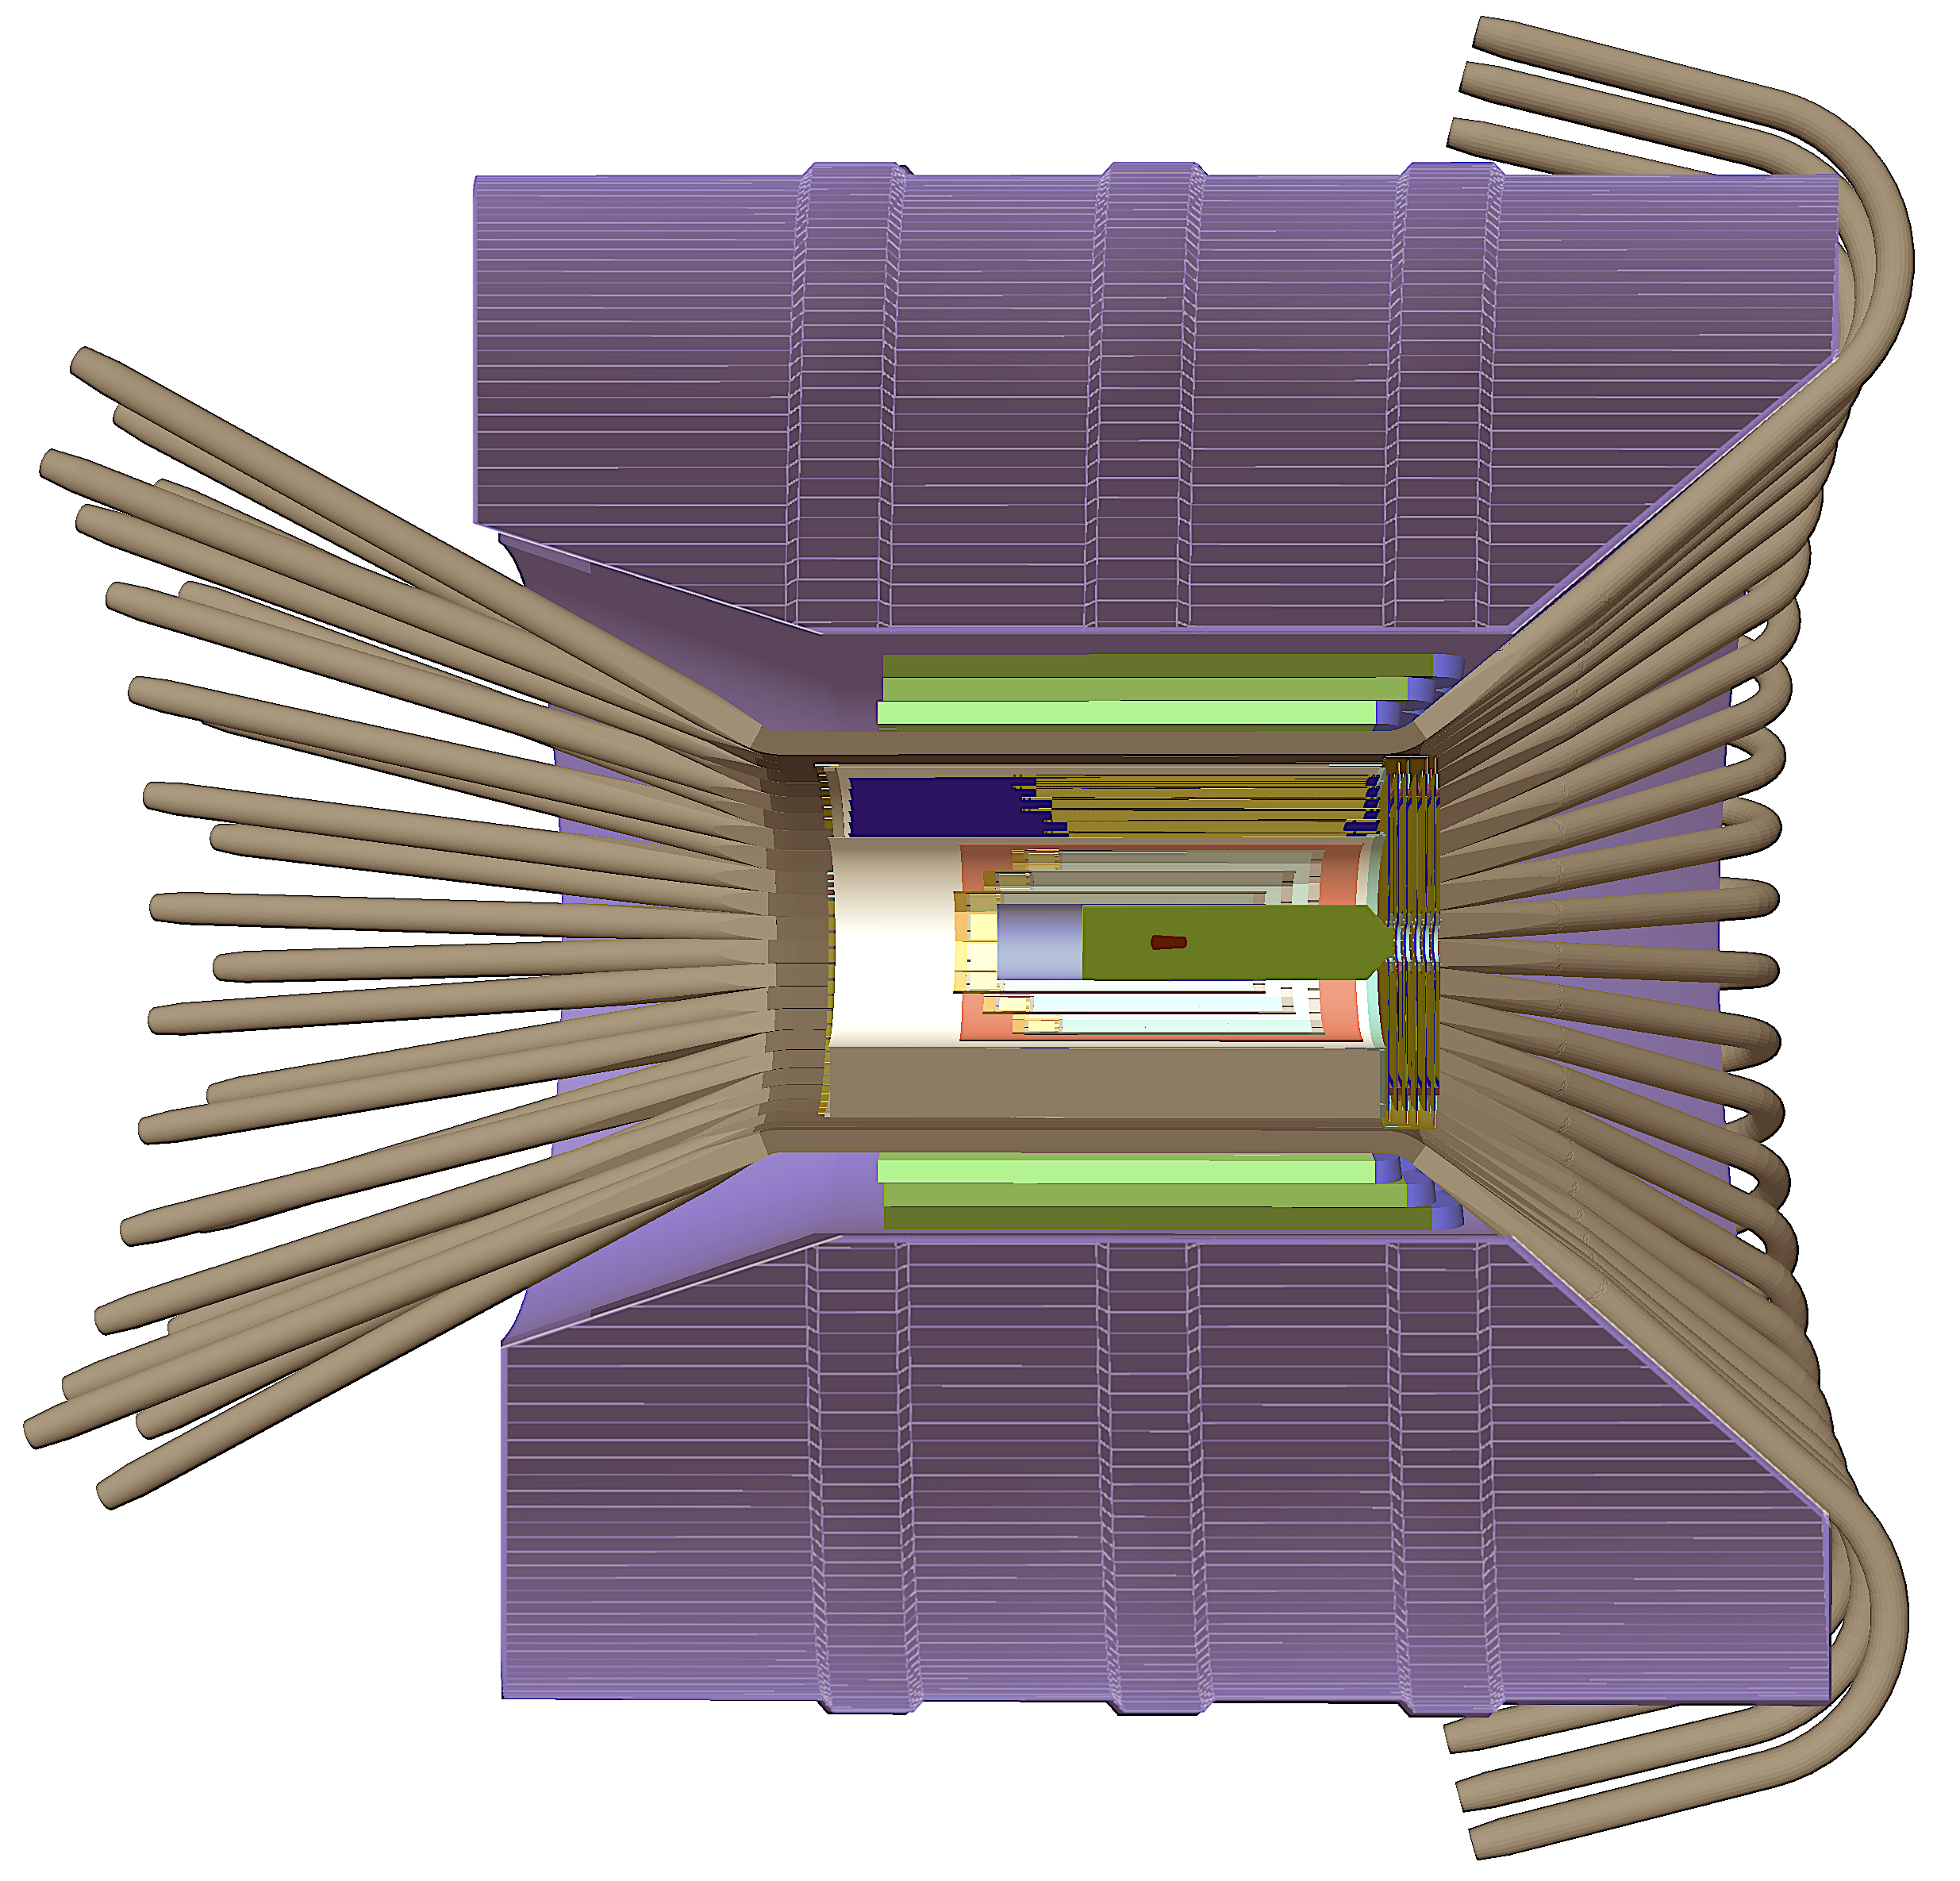
\includegraphics[width=0.98\columnwidth,keepaspectratio]{img/solenoid.png}
   \caption{An 11 GeV electron beam is impinging on a 5 cm liquid hydrogen target. At the full $10^{35} cm-2s-1$ luminosity, this correspond to
            124,000 electrons in a 250 ns window. Normally this would produce a storm of Moeller electrons that would saturate any detector in the forward or central
				region. However the solenoid focus all of the Moeller electrons along the beam line, providing a most effective shield for CLAS12.
            }
	\label{fig:solenoid}
\end{figure}

The torus geometry is imported from the engineering CAD model through 54 tessellated volumes. Among the volumes:

\begin{itemize}
	\item the bore heat shield and hub components
	\item the back and front hub steel plates
	\item the stainless steel coil vacuum jackets
	\item the torus coils containing the wires, represented by copper volumes in geant4
\item internal shielding around the hub, made by tungsten cylinders (blue in \F{torus})
\end{itemize}

The torus hub is protected from the beampipe background with additional tungsten shielding.
The torus geometry is shown in \F{torus}.

\begin{figure}
	\centering
	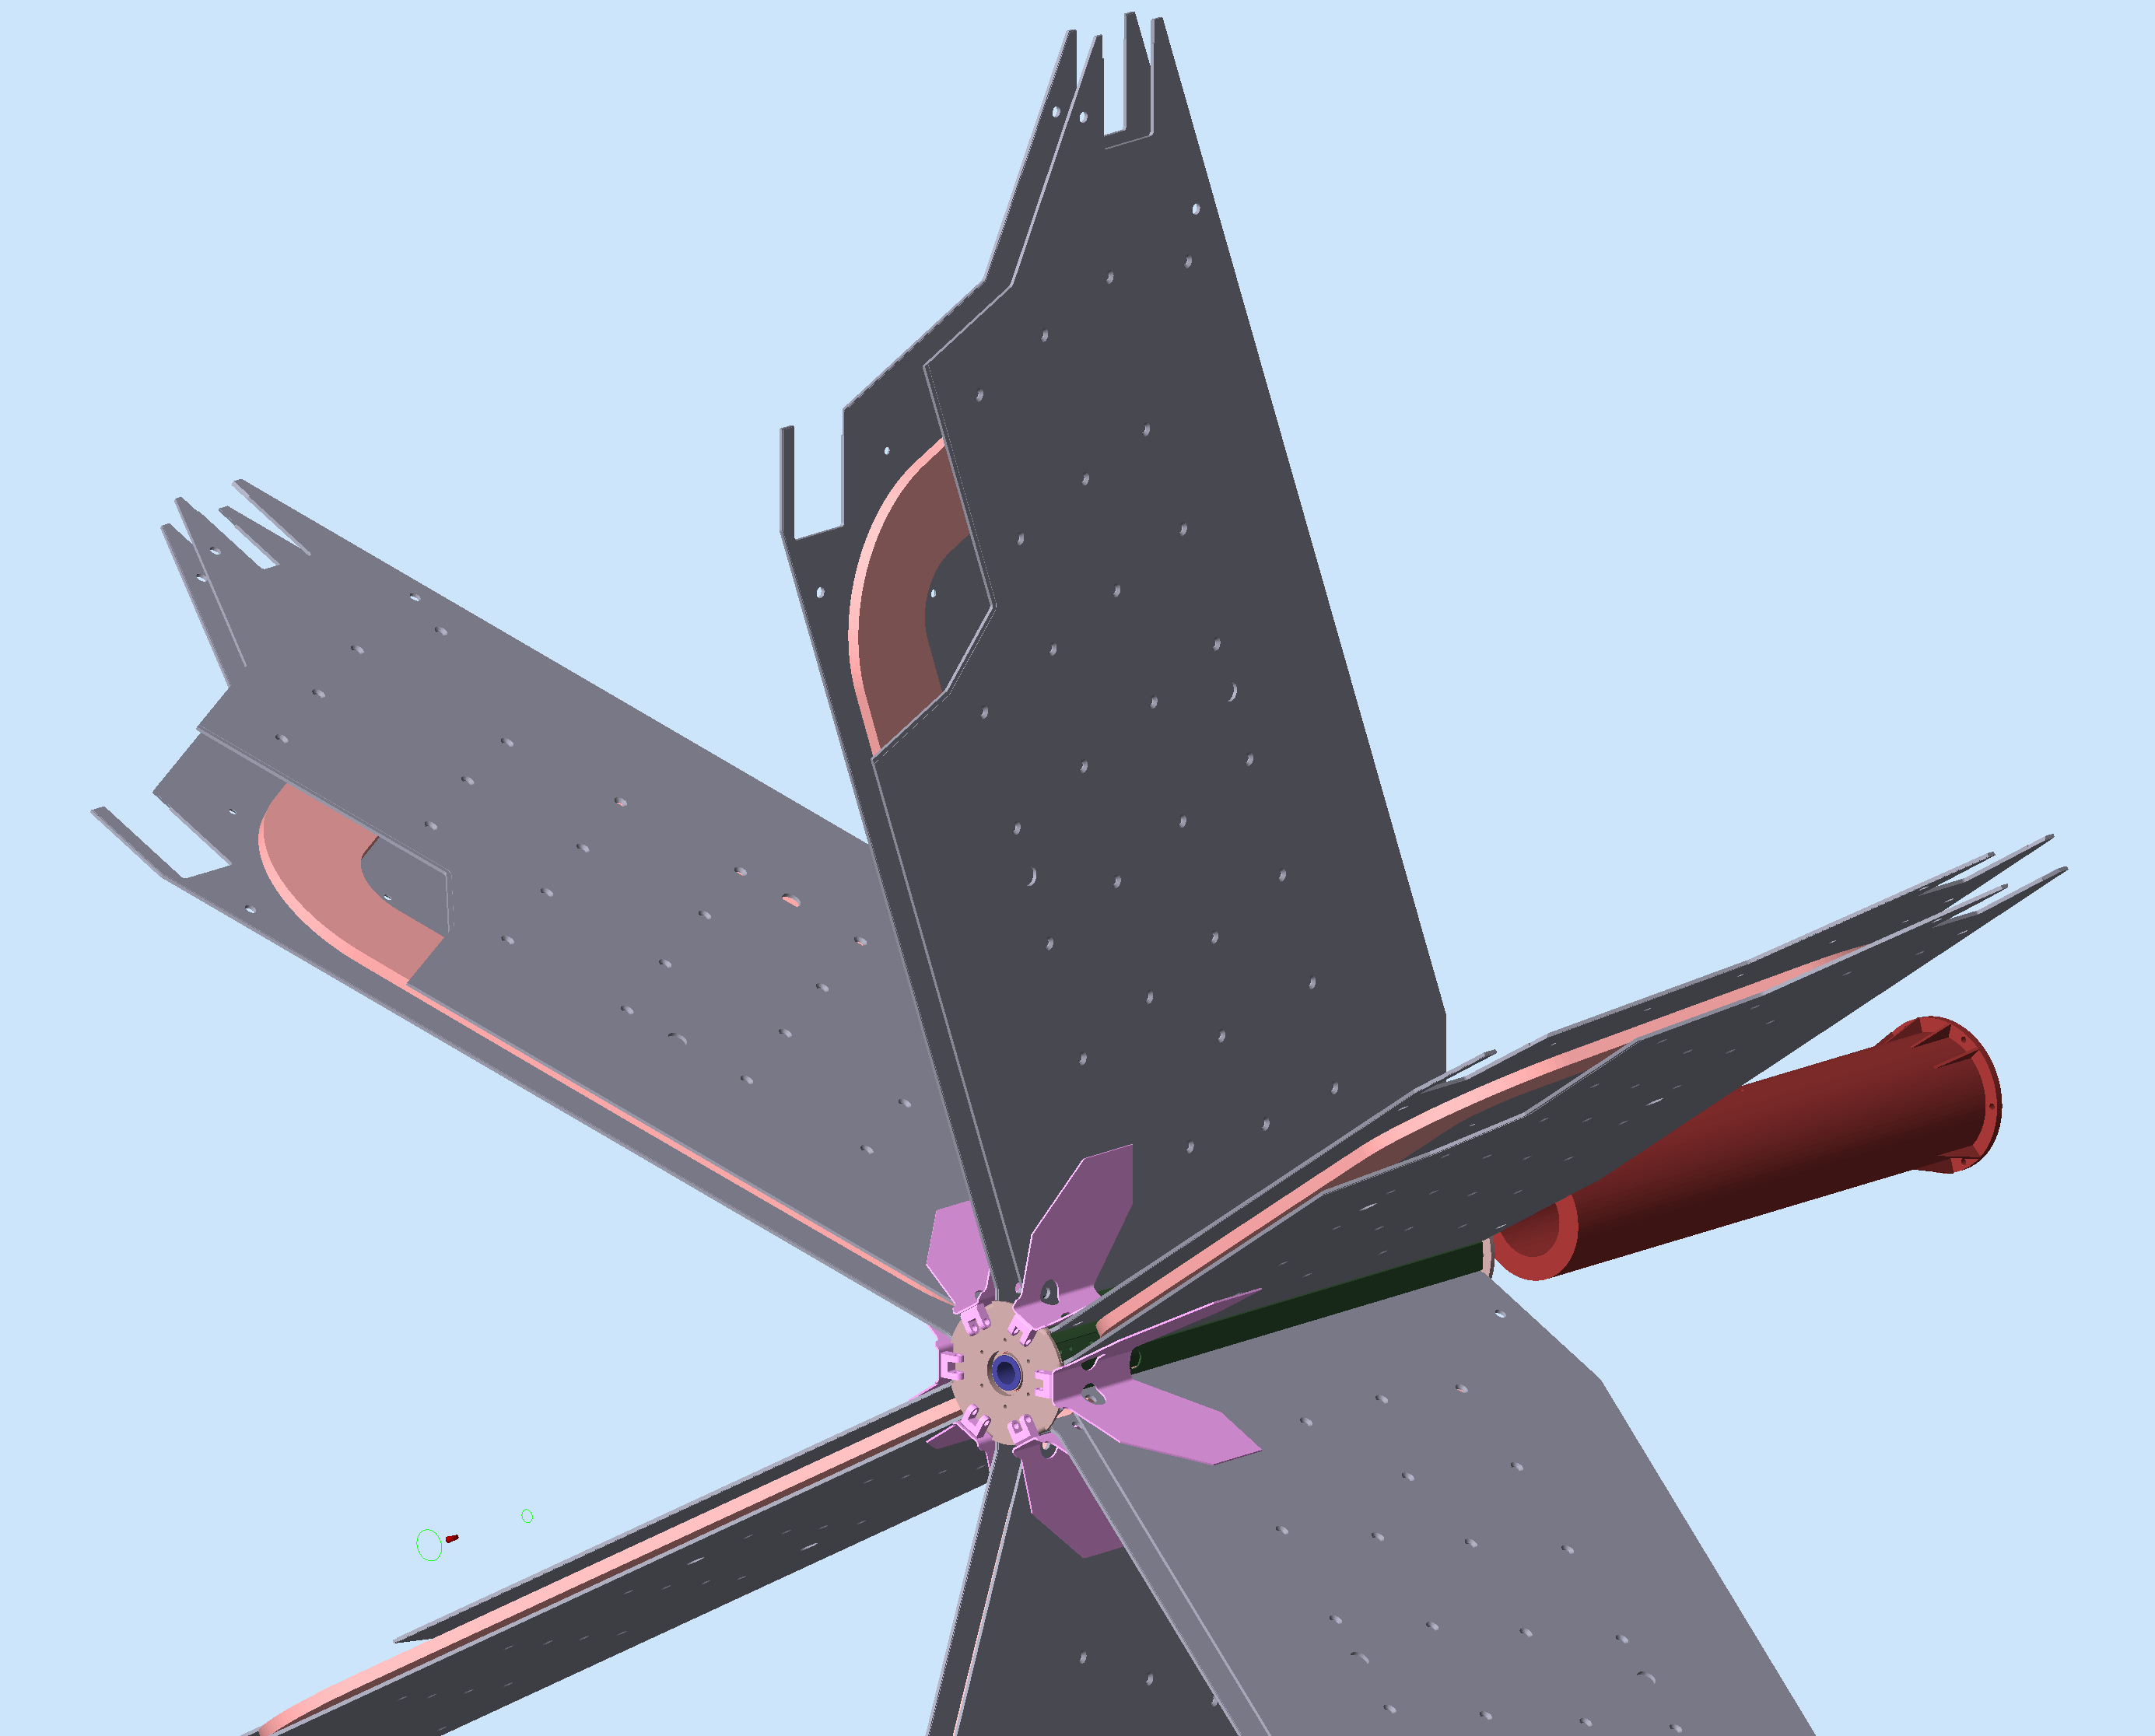
\includegraphics[width=0.95\columnwidth,keepaspectratio]{img/torusGeometry.png}
	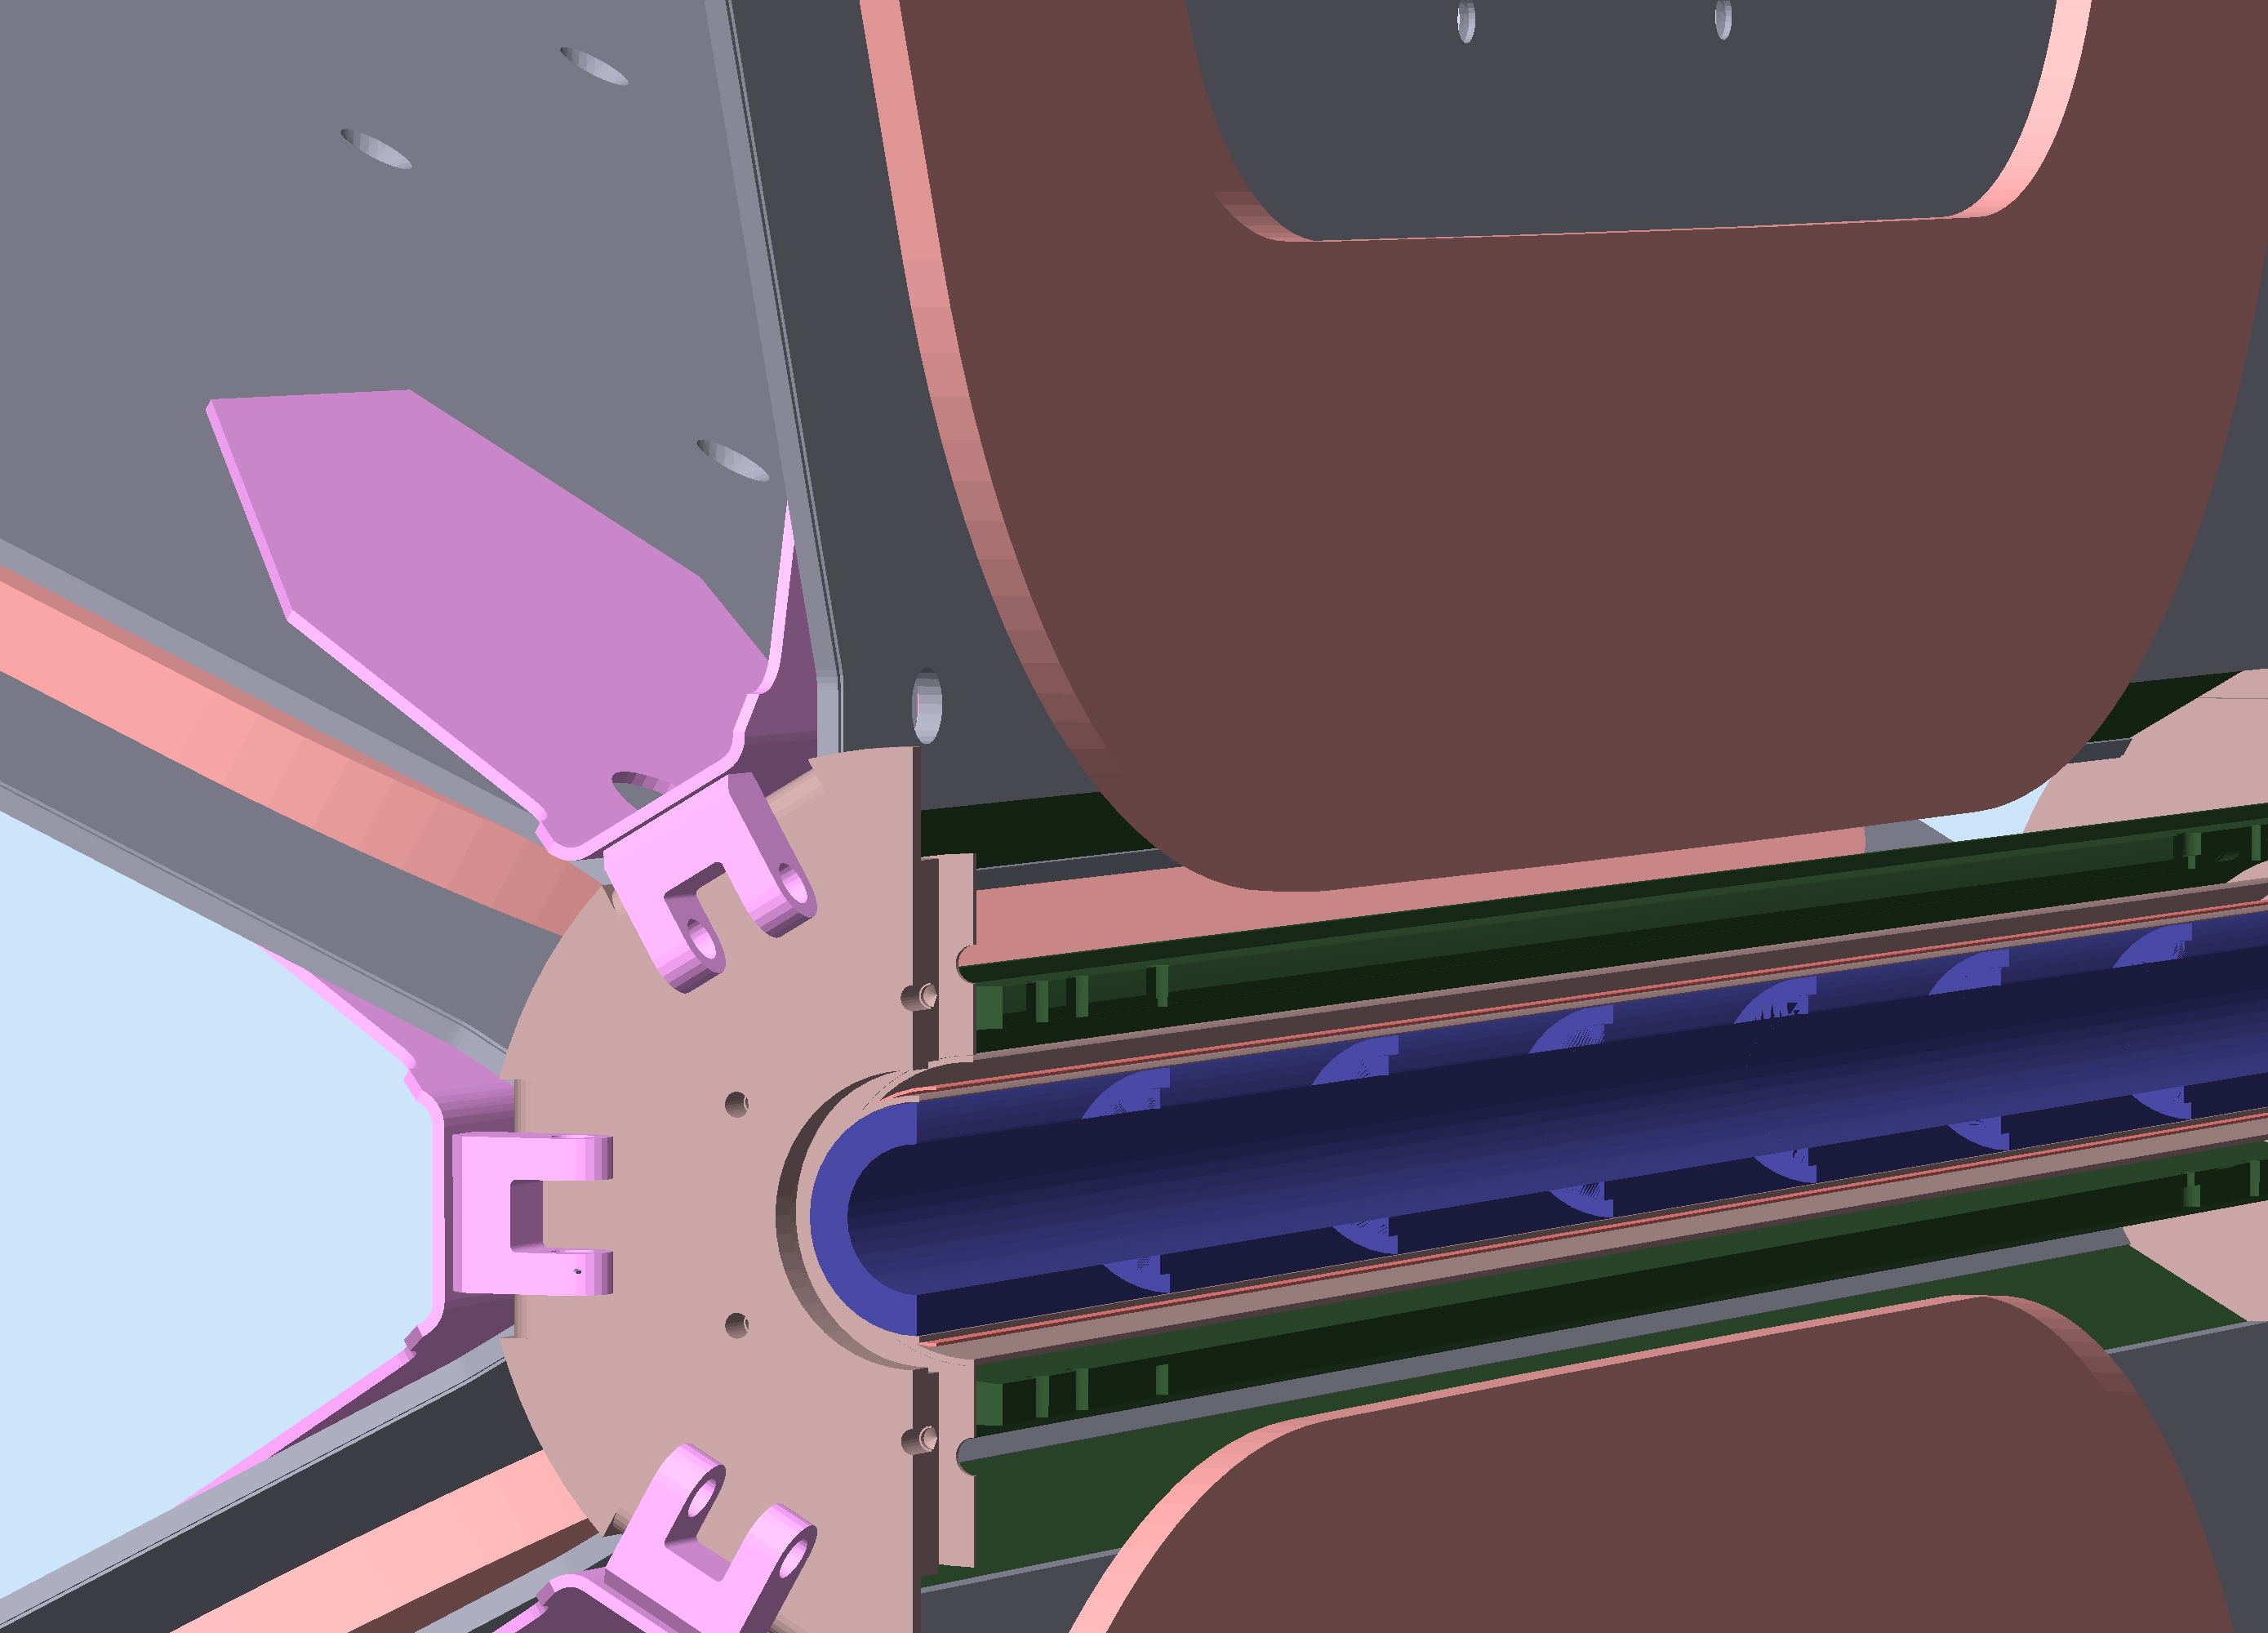
\includegraphics[width=0.95\columnwidth,keepaspectratio]{img/torusDetail.png}
	\caption{Top: the GEMC implementation of the torus hardware. The volumes are imported from the CAD engineering model.
            The stainless steel vacuum jacket embeds the geant4 coil volumes.
				Bottom: a section view of the torus in the vicinity of the beamline. The warm and cold hub are visible, along with the
				tungsten shielding (blue colors).}
	\label{fig:torus}
\end{figure}


\subsection{Magnetic Field Maps} \label{clas12FieldMaps}


The field maps are imported into the simulation using ascii files. Both fields can be scaled by an arbitrary number.
Both fields are defined in the Hall B coordinate system and both can be shifted and tilted by additional delta amounts.

\subsubsection{Solenoid}
The solenoid field map has cylindrical symmetry around the z- axis, so the map used in the simulation is defined in the transverse / longitudinal plane
and then rotated when requested by the Geant4 navigation. The integration method used in the simulation is the Runge-Kutta 4.

The solenoid field near the target is parallel to the z-axis and its uniformity was measured to be 318 ppm over a 25mm diameter and 40mm long cylindrical volume.
The field map grid is made by 600 points in the transverse coordinate, from 0 to 3m and by 1200 points
along the z-axis, from \mbox{-3m} to 3m.
The field grid values are linearly interpolated to the (x,y,z) coordinate requested by geant4.

Table \ref{tab:solMap} shows the field map ascii data structure.


\begin{table}[h]
	\begin{center}
		\begin{tabular}{| c | c | c | c |}
			T (m)  & Z (m) &  $B_T $  & $ B_L $ \\
			\hline
          0.005  &  -0.025 & 0.000013  & 5.000880 \\
          0.005  &  -0.020 & 0.000044  & 5.000822 \\
          0.005  &  -0.015 & 0.000073  & 5.000704 \\
          0.005  &  -0.010 & 0.000101  & 5.000529 \\
          0.010  &  -0.025 & 0.000028  & 5.000928 \\
          0.010  &  -0.020 & 0.000089  & 5.000867 \\
          0.010  &  -0.015 & 0.000148  & 5.000747 \\
          0.010  &  -0.010 & 0.000203  & 5.000570 \\
		\end{tabular}
	\end{center}
\caption{Solenoid ascii field map values around the target. T is the transverse coordinate $\sqrt{(x^2+y^2)}$ and z is the longitudinal coordinate.
            The solenoid field is centered at Z=0, the location of the center of the target. The field values are in Tesla.}\label{tab:solMap}
\end{table}

\subsubsection{Torus}
The torus field can be imported using a symmetric map or a full 3D map.
The symmetric map is defined in half the CLAS12 sector. It is symmetric around the sector mid-plane and copied in each sector
when requested by the Geant4 navigation. The 3D map covers the entire cartesian space and accounts for field deviations due to coil
movements or imperfections \cite{GhoshalSolenoid}.


The field map has 251 points along the z-axis, from 1m to 3m. It has 2501 points in the transverse coordinate, from 0 to 5m.
It has 16 azimuthal points from $0$ to $30^0$. The field grid values are linearly interpolated to the (x,y,z) coordinate requested by geant4.

The torus field in mid sector is perpendicular to the z-axis and is typically $2.058$ Tesla.
Table \ref{tab:torMap} shows the field map ascii data structure.

\begin{table}[h]
	\begin{center}
		\begin{tabular}{| c | c | c | c | c | c | }
         $\phi$ (deg) & T (m)    & Z (m)    &  $B_x $  &    $B_y$    & $B_z$\\
			\hline
          0.0         &  190.0   &  338.0   &  0       &     0.451275 &  0 \\
          0.0         &  190.0   &  340.0   &  0       &     0.450136 &  0 \\
          0.0         &  190.0   &  342.0   &  0       &     0.448789 &  0 \\
          0.0         &  190.0   &  344.0   &  0       &     0.447235 &  0 \\
          0.0         &  190.0   &  346.0   &  0       &     0.445472 &  0 \\
          0.0         &  190.0   &  348.0   &  0       &     0.443502 &  0 \\
          0.0         &  190.0   &  350.0   &  0       &     0.441323 &  0 \\
          0.0         &  190.0   &  352.0   &  0       &     0.438935 &  0 \\
		\end{tabular}
	\end{center}
	\caption{Torus ascii field map values near mid-sector. T is the transverse coordinate $\sqrt{(x^2+y^2)}$ and z is the longitudinal coordinate.
            The field values are in Tesla.}\label{tab:torMap}
\end{table}


\subsubsection{Geometry Location on GitHub}
The Github location of the GEMC perl API script for the solenoid and the torus CAD volumes is \url{https://github.com/gemc/detectors/tree/master/clas12/magnets}.

